\section{Interior Point Methods (IPM)}
\label{Sec:ipm}

% InteriorPoint_QP_beamer.tex
% 4-slide Beamer presentation explaining interior-point techniques for a convex quadratic program.
% Save as InteriorPoint_QP_beamer.tex and compile with pdflatex (or lualatex/xelatex).



% Slide 1: Problem statement + KKT
\begin{frame}{A Primer on IPM for convex QP}
  \begin{block}{Convex QP}
Consider the convex quadratic program in standard form:
\begin{align*}
  &\min_{x\in\mathbb{R}^n} \; f(x) := \tfrac{1}{2}x^T Q x + c^T x\\
  &\text{subject to }\; A x = b, \quad x \ge 0,
\end{align*}
where $Q\succeq 0$, $A\in\mathbb{R}^{m\times n}$.

First-order (KKT) conditions (existence of multipliers $y,z$):
\begin{align*}
  Qx + c + A^T y - z &= 0 \quad (\text{stationarity})\\
  Ax - b &= 0 \quad (\text{primal feasibility})\\
  X Z e &= 0,\quad x\ge0,\ z\ge0 \quad(\text{complementarity})
\end{align*}
where $X=\mathrm{diag}(x)$, $Z=\mathrm{diag}(z)$, $e$ is the vector of ones.
\end{block}
\begin{block}{Interior-point idea}
   Enforce strict positivity $x>0, z>0$ and drive $XZe=\mu e$ to zero along the \emph{central path} as $\mu\downarrow0$.
\end{block}

\end{frame}

% Slide 2: Barrier method + Newton step + figure
\begin{frame}{A Primer on IPM for convex QP}
  
\only<1>
{
  \begin{block}{Barrier formulation and Newton steps}
  Use a logarithmic barrier to keep $x>0$:
\[
  \phi_\mu(x)=\tfrac{1}{2}x^T Q x + c^T x - \mu \sum_{i=1}^n \log x_i
\]
with equality constraints $Ax=b$. For fixed $\mu>0$ solve
\[\min_{x>0}\; \phi_\mu(x) \quad\text{s.t. } Ax=b.\]
\end{block}
The perturbed KKT conditions for $\mu>0$ are:
\begin{align*}
  Qx + c + A^T y - z &= 0, \\
  Ax - b &= 0, \\
  XZe &= \mu e.
\end{align*}
}
\only<2>{
We linearize these equations at $(x,y,z)$ to get the Newton system for $(\Delta x, \Delta y, \Delta z)$:
\[
  \begin{bmatrix}
    Q & A^T & -I \\
    A & 0   & 0   \\
    Z & 0   & X
  \end{bmatrix}
  \begin{bmatrix}
    \Delta x \\
    \Delta y \\
    \Delta z
  \end{bmatrix}
  = -\begin{bmatrix}
    r_d \\
    r_p \\
    r_c
  \end{bmatrix},
\]
where
\begin{align*}
  r_d &= Qx + c + A^T y - z,\\
  r_p &= Ax - b,\\
  r_c &= XZe - \mu e.
\end{align*}
This 3-block structure is the foundation of primal--dual interior-point methods.
Take a damped Newton step and project back to positive orthant with step-length chosen to maintain $x>0$.
}
% \only<2>
% {
% \vspace{2mm}
% \textbf{Figure: feasible region (linear constraints) and central path for a QP}
% \begin{center}
% \begin{tikzpicture}[scale=1]
%   % feasible polytope (two inequality lines) + ellipse objective contours
%   \filldraw[fill=gray!8] (0.3,0.4) -- (3.2,0.2) -- (3.7,2.8) -- (0.6,2.6) -- cycle;
%   % axes
%   \draw[->] (0,0) -- (4,0) node[right] {$x_1$};
%   \draw[->] (0,0) -- (0,3) node[above] {$x_2$};
%   % objective contours (ellipses)
%   \draw (1.8,1.4) ellipse (1.6 and 0.8);
%   \draw (1.8,1.4) ellipse (1.2 and 0.6);
%   \draw (1.8,1.4) ellipse (0.8 and 0.35);
%   % central path curve
%   \draw[thick,->,red] plot [smooth,domain=0:1] ( {0.5+3*\x^1.2}, {2.5-1.6*\x^0.9} ) node[right]{central path};
%   % current iterates
%   \foreach \t in {0.12,0.28,0.46,0.7,0.9}{\filldraw[black] ({0.5+3*\t^1.2},{2.5-1.6*\t^0.9}) circle (1.8pt);}
%   % optimum
%   \filldraw[blue] (1.8,1.4) circle (2.4pt) node[right] {optimal $x^*$};
% \end{tikzpicture}

% \end{center}
%}
\end{frame}


\begin{frame}{Full Newton step for primal--dual system}
The perturbed KKT conditions for $\mu>0$ are:
\begin{align*}
  Qx + c + A^T y - z &= 0, \\
  Ax - b &= 0, \\
  XZe &= \mu e.
\end{align*}
We linearize these equations at $(x,y,z)$ to get the Newton system for $(\Delta x, \Delta y, \Delta z)$:
\[
  \begin{bmatrix}
    Q & A^T & -I \\
    A & 0   & 0   \\
    Z & 0   & X
  \end{bmatrix}
  \begin{bmatrix}
    \Delta x \\
    \Delta y \\
    \Delta z
  \end{bmatrix}
  = -\begin{bmatrix}
    r_d \\
    r_p \\
    r_c
  \end{bmatrix},
\]
where
\begin{align*}
  r_d &= Qx + c + A^T y - z,\\
  r_p &= Ax - b,\\
  r_c &= XZe - \mu e.
\end{align*}
This 3-block structure is the foundation of primal--dual interior-point methods.
\end{frame}


% Slide 3: Central path illustration
\begin{frame}{Illustration of the central path}
\textbf{Definition:} The \emph{central path} is the trajectory of strictly feasible points $(x(\mu), y(\mu), z(\mu))$ satisfying
\[
Qx(\mu) + c + A^T y(\mu) - z(\mu) = 0, \quad Ax(\mu) = b, \quad X(\mu) Z(\mu)e = \mu e,\; \mu>0.
\]
As $\mu \to 0$, the path converges to the optimal solution $(x^*,y^*,z^*)$.

\vspace{2mm}
\textbf{Geometric intuition:}
\begin{itemize}
  \item Each $\mu$ defines a barrier problem that smooths the feasible region.
  \item The central path traces the minimizers of these smoothed problems.
  \item Interior-point methods follow this path using Newton directions.
\end{itemize}

% \vspace{2mm}
% \begin{center}
% \begin{tikzpicture}[scale=1]
%   % axes
%   \draw[->] (0,0) -- (4.5,0) node[right] {$x_1$};
%   \draw[->] (0,0) -- (0,3.2) node[above] {$x_2$};
%   % feasible region (wedge)
%   \draw[fill=gray!10] (0.5,0.5) -- (4,0.5) -- (4,2.5) -- (0.5,2.5) -- cycle;
%   \node at (3.4,2.7) {feasible region};
%   % objective contours (ellipses)
%   \draw (2,1.4) ellipse (1.6 and 0.8);
%   \draw (2,1.4) ellipse (1.2 and 0.6);
%   \draw (2,1.4) ellipse (0.8 and 0.35);
%   % central path (smooth curve)
%   \draw[thick,red,->] plot [smooth,domain=0:1] ( {0.6+2.8*\x^1.2}, {2.4-1.7*\x^0.9} );
%   % arrows and labels for mu values
%   \foreach \m/\t in {1.0/0.1,0.3/0.4,0.1/0.7,0.03/0.9}{
%     \filldraw[red] ({0.6+2.8*\t^1.2},{2.4-1.7*\t^0.9}) circle (1.5pt);
%     \node[anchor=west,scale=0.8] at ({0.6+2.8*\t^1.2+0.1},{2.4-1.7*\t^0.9}) {$\mu=\m$};}
%   % optimal point
%   \filldraw[blue] (2,1.4) circle (2pt) node[right] {$x^*$};
% \end{tikzpicture}
% \end{center}

\vspace{1mm}
\textbf{Interpretation:} As $\mu$ decreases, the minimizer moves smoothly along the red curve toward the boundary optimum.
\end{frame}

% Slide: Central path in the positive orthant (as in Nocedal & Wright)
\begin{frame}{Central path in the positive orthant (boundary optimum)}
The central path for a problem with $x \ge 0$ approaches the boundary smoothly
as $\mu \to 0$. The iterates remain strictly positive until convergence.

\begin{center}
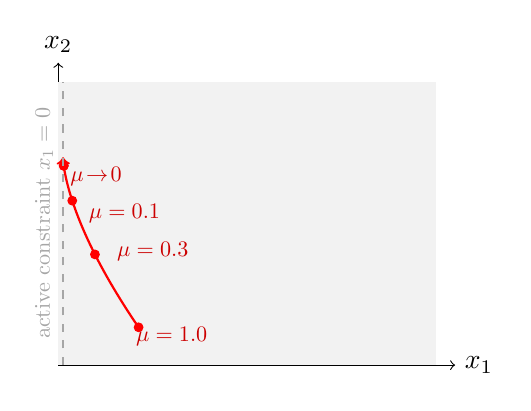
\begin{tikzpicture}[scale=1.2]
  % Axes
  \draw[->] (0,0) -- (4.2,0) node[right] {$x_1$};
  \draw[->] (0,0) -- (0,3.2) node[above] {$x_2$};
  
  % Feasible region: positive orthant
  \fill[gray!10] (0,0) rectangle (4,3);

  % % Objective contours (ellipses)
  % \foreach \a in {0.6,0.9,1.2,1.5}{
  %   \draw[gray!70] (2.5,1.5) ellipse (1.8/\a and 1.0/\a);
  % }

  % Central path approaching x1=0 boundary
  \draw[thick,red,->,domain=0:1,smooth,variable=\t]
    plot ({0.8*(1-\t)^2 + 0.05},{2.2 - 1.8*(1-\t)^1.3});

  % Points along path (decreasing mu)
  \foreach \m/\t in {1.0/0.0,0.3/0.35,0.1/0.65,0.03/0.9,0.01/0.9}{
    \filldraw[red] ({0.8*(1-\t)^2 + 0.05},{2.2 - 1.8*(1-\t)^1.3}) circle (1.3pt);
  }

  % Labels for mu values
  \node[red!80!black,scale=0.8] at (0.4,2.0) {$\mu\!\to\!0$};
  \node[red!80!black,scale=0.8] at (0.7,1.6) {$\mu=0.1$};
  \node[red!80!black,scale=0.8] at (1.0,1.2) {$\mu=0.3$};
  \node[red!80!black,scale=0.8] at (1.2,0.3) {$\mu=1.0$};

  % Optimal point on the boundary
  
  % \filldraw[blue] (0.0,2.1) circle (2pt);
  % \node[anchor=west,blue,scale=0.9] at (0.0,2.1) {$x^* = (0, x_2^*)$};

  % Annotate the active constraint line
  \draw[dashed,gray!70] (0.05,0) -- (0.05,3);
  \node[gray!70,scale=0.8,rotate=90] at (-0.15,1.5) {active constraint $x_1=0$};

\end{tikzpicture}
\end{center}


\textbf{Interpretation:}
As $\mu \downarrow 0$, $x_1(\mu) \to 0$ and the iterates approach the boundary while maintaining strict positivity, ensuring well-defined Newton steps.
\end{frame}
% Slide 4: Primal-dual IPM, residuals and convergence
\begin{frame}{Primal--dual interior-point method \& practical notes}
Primal--dual methods work with both primal and dual variables and maintain perturbed complementarity:
\[XZ e = \sigma \mu e,\quad \mu=\frac{x^T z}{n},\quad 0<\sigma\le1.
\]
A common predictor--corrector algorithm (Mehrotra) computes a predictor (affine-scaling) step, estimates a \(\sigma\), then corrects to stay close to the central path.

Key practical points:
\begin{itemize}
  \item Use sparse symmetric linear algebra to solve the Newton/KKT system efficiently.
  \item Choose step-lengths to keep iterates positive; use Mehrotra predictor-corrector for fast practical convergence.
  \item Convergence: polynomial worst-case complexity (typically 30--60 iterations for large QPs in practice).
\end{itemize}

Interior-point methods follow the central path using Newton steps on a barrier-regularized KKT system; primal--dual variants maintain both primal and dual feasibility and usually reach high accuracy in few iterations.
\end{frame}





\begin{frame}
  \frametitle{Interior Point Methods for frictional contact}
  \begin{block}{PhD thesis of Hoang Minh Nguyen(2025), with Paul Armand}
   Perturbation of the complementarity condition with a barrier parameter $\tau$\\[2mm]
  
    \begin{columns}[c]
        % \small
      \begin{column}{.5\textwidth}
            \begin{equation*}
              \begin{array}{c}
                \text{ \tr{Original problem}} \\[2mm]
                    M v + f = H^\top r \\
                    H v + w + se = \tilde{u} \\
                    s = \norm{\tilde{u}_\t} \\
                    \tilde{u} \circ r = 0  \\
                    (\tilde{u}, r) \in K^2
                \end{array}
            \end{equation*}
        \end{column}
        \hspace{-1cm}
        \begin{column}{.5\textwidth}
            \begin{equation}
                \label{eq:per-incre-prob}
                \begin{array}{c}
                    \text{ \tr{Perturbed problem}} \\[2mm]
                    M v + f = H^\top r \\
                    H v + w + se = \tilde{u} \\
                    s = \norm{\tilde{u}_\t} \\
                    \tilde{u} \circ r = 2\tau e \\
                    (\tilde{u}, r) \in \mbox{int}(K^2)
                \end{array}
            \end{equation}
        \end{column}
      \end{columns}
    \end{block}
    
    \begin{block}{Convex case ($s$ fixed)}
      IPM is able to solve very accurately and efficiently the problem with a given $s := \| u_\t \|$ even when $H$ is rank-deficient (see \cite{acary:hal-03913568}).\\ Special care of sparse linear systems and conditioning with Nesterov-Todd scaling.
    \end{block}
  \ding{220} Extension to general frictional contact problems: nonsmooth interior point method

  
\end{frame}

\begin{frame}{Nonsmooth Interior-Point Method (NIPM)}
    % \vspace{-0.3cm}

    \tr{Slater's assumption (SA)} \quad $\exists v \in \nbR^m$ \quad such that \quad $Hv+w \in \mbox{int}({K})$
    \begin{theorem}
        \vspace{-5pt}
        \begin{enumerate}
            \item Under SA, for each $\tau > 0$, the perturbed problem \eqref{eq:per-incre-prob} has a solution $(v_\tau,\tilde{u}_\tau,r_\tau,s_\tau)$ \\[6pt]
            \item Under SA, there exists an analytic central path $\{(v_\tau,\tilde{u}_\tau,r_\tau,s_\tau): \tau>0\}$, which converges to a solution of the original problem
        \end{enumerate}
      \end{theorem}
      Proof: Fixed point  Brouwer's Theorem and curve selection lemma in semi-algebraic analysis.
      
      \begin{block}{Main theoretical outcome}
        \begin{itemize}
        \item Alternative proof of solution existence for $\mathrm{FC/I}(M,H,f,w,\mu)$
        \item  The central path is not necessarily unique !
        \end{itemize}
      \end{block}
\end{frame}


\begin{frame}{Nonsmooth Interior-Point Method (NIPM) - Linearization}
  \begin{block}{{Iterations and Jacobian matrix }}
    \begin{columns}[c]
      \begin{column}{.5\textwidth}
        \begin{equation*}
          G:=\begin{bmatrix} Mv+f-H^\top r \\ Hv+w-\tilde{u}+se \\ s - \norm{\tilde{u}_\t} \\ \tilde{u} \circ r \end{bmatrix}
          = \begin{bmatrix} 0 \\ 0 \\ 0 \\ 2\tau e \end{bmatrix}
        \end{equation*}
        \quad
      \end{column}
      \begin{column}{.5\textwidth}
        \begin{equation*}
          J:=\begin{bmatrix} M & -H^\top & 0 & 0 \\ H & 0 & -I & e \\ 0 & 0 & -L & 1 \\ 0 & \tilde{U} & R & 0 \end{bmatrix}
        \end{equation*}
        \quad
      \end{column}
    \end{columns}
    % \vspace{0.1cm}
     where $L = \begin{pmatrix} 0 & \partial \norm{\tilde{u}_\t}^\top \end{pmatrix}$, \quad $\mbox{with } \partial \norm{\tilde{u}_\t} = \begin{cases} \frac{\tilde{u}_\t}{\norm{\tilde{u}_\t}} & \mbox{if } \tilde{u}_\t \neq 0 \\ d \in \mathbb B & \mbox{if } \tilde{u}_\t = 0  \end{cases}$ (unit ball $\mathbb B$)
  \end{block}
    %
  \begin{block}{Linear system and Mehrotra's-Like algorithm}
    $$J \, d = -G + \left[ \begin{matrix} 0 \\ 0 \\ 0 \\ 2\sigma \tau e \end{matrix}\right]$$ predictor-corrector scheme $\sigma \in (0,0.5)${\small: centralization parameter}
  \end{block}
   \begin{block}{Stopping test}
     $$\max\left\{ \; \|Hv+w-\tilde{u}\|_\infty, \; \|Mv+f-H^\top r\|_\infty, |s - \norm{\tilde{u}_\t}|, \; \|\tilde{u} \circ r\| \; \right\}  \; \leq \; \mbox{tol}$$
   \end{block}
 \end{frame}

 \begin{frame}
   \frametitle{Nonsmooth Interior-Point Method (NIPM)}
   
   \begin{algorithm}[H]
     \scriptsize
  \caption{Mehrotra type Nonsmooth Interior Point Method (NIPM)}
  \label{alg:IP}
  %\hspace*{\algorithmicindent} 
  \textbf{Parameters:} Choose a starting point $(v,r,u,s)$ such that $(r,u)\in{\rm int}({\cal K}^2)$. Choose $\eta_1\in(0,1)$, $\eta_2\geq 1$, $\eta_3\geq 1$, $\gamma_1\in(0,1)$, $\gamma_2\in (0,1-\gamma_1)$, $c_1\geq 1$, $c_2\in(0,1)$, $\rm{tol}>0$ and set $\gamma = 0.99$;
  \begin{algorithmic}[1]
    \State\label{step1}{\bf if} the stopping criterion is satisfied {\bf then} return $(v,r,u,s)$ as solution of \eqref{eq:math-model}; 
    \State\label{step2} Set $\tau\leftarrow u^\top r / n$;
    \State\label{step3} {\bf if} $\|s-\ell(u)\|_2 \geq c_1 \| u \circ r\|_2$ {\bf then} set $\sigma \leftarrow 0.998$, $d^u_a \circ d^r_a \leftarrow 0$ and go to \ref{step10},
    \State\label{step4} {\bf else} compute $d_a=(d^v_a,d^r_a,d^u_a,d^s_a)$ solution of
    \begin{displaymath}
      J(v,r,u,s) d_a = -G(v,r,u,s);
    \end{displaymath}
    \State\label{step5} Find the greatest $\alpha_a\in(0,1]$ such that $(r,u)+\alpha_a(d_a^r,d_a^u) \in {\cal K}^2$;
    \State\label{step6} Set $\tau_a \leftarrow  (u+\alpha_a d^u_a)^\top(r+\alpha_a d^r_a)/n$;
    \State\label{step7} {\bf if} {$\tau>\eta_1$}\,  {\bf then} set $\beta\leftarrow \max\{1,\eta_2 \alpha_a^2\}$\, {\bf else} set $\beta \leftarrow \eta_3$;
    \State\label{step8} Set $\sigma \leftarrow 0.998\min\{1,(\tau_a/\tau)^\beta\}$;
    \State\label{step9} {\bf if}  $\sigma \geq c_2$  {\bf then} set $d^u_a \circ d^r_a \leftarrow 0$;
    \State\label{step10} Compute $d=(d^v,d^r,d^u,d^s)$ solution of
    \begin{equation}
      \label{eq:JdG}
      J(v,r,u,s) d = -G(v,r,u,s)+\left[\begin{smallmatrix} 0\\0\\-d^u_a \circ d^r_a + \sigma\tau e\\ 0\end{smallmatrix}\right]
    \end{equation}
    \State\label{step11} Find the greatest $\alpha\in(0,1]$ such that $(r,u)+\alpha(d^r,d^u) \in (1-\gamma)(r,u) + {\cal K}^{2}$;
    \State\label{step12} Set $\gamma \leftarrow \gamma_1 + \alpha \gamma_2$;
    \State\label{step13} Set $(v,r,u,s) \leftarrow (v,r,u,s) + \alpha (d^v, d^r,d^u,d^s)$ and goto \ref{step1}.
   \end{algorithmic}
 \end{algorithm}

 \end{frame}


\begin{frame}
  \frametitle{Nonsmooth Interior-Point Method (NIPM)}
   \begin{center}
    \includegraphics[height=0.7\textheight]{./figure/IPM/solver_performance_11_100.jpg}
  \end{center}
  \begin{block}{Problem's size $11\leq n \leq 100$}
    IPM (GFC3D) outperforms NSGS and ADMM in terms of efficiency and robustness
  \end{block}
\end{frame}
\begin{frame}
  \frametitle{Nonsmooth Interior-Point Method (NIPM)}
  
  \begin{center}
    \includegraphics[height=0.7\textheight]{./figure/IPM/solver_performance_1000_.jpg}
  \end{center}

  \begin{block}{Problem's size $1000\leq n $}
    IPM (GFC3D) suffers from robustness
  \end{block}
  
\end{frame}

\begin{frame}{Nonsmooth Interior-Point Method (NIPM) - failures}
    \vspace{-0.1cm}
    % \begin{exampleblock}{Questions}
    %     {\color{greenexampleblock}$\bullet$} Why we require such high accuracy, specifically up to $10^{-14}$ ? \\
    %     $\to$ To ensure an accurate identification of contact status \\[6pt]
    %     {\color{greenexampleblock}$\bullet$} What is the cause of failures ?
    % \end{exampleblock}
    \begin{exampleblock}{Failure \#1: {\color{black} A special shape of the central path}}
        \begin{center}
            \includegraphics[width=0.495\linewidth]{./figure/IPM/images/ncv_fail1a.png}
            \includegraphics[width=0.495\linewidth]{./figure/IPM/images/ncv_fail1b.png}
        \end{center}
        \begin{center}
        Solution: \quad {\color{blue} $r$}$^\times${\color{blue} $\in \mbox{int}({K})$}, \quad {\color{red} $\tilde{u}$}$^*${\color{red} $= 0$} \quad (sticking)
        \end{center}
    \end{exampleblock}
    This shape of the central path can cause iterates to get stuck on the boundary, which is not the correct position for the solution.
\end{frame}




\begin{frame}{Nonsmooth Interior-Point Method (NIPM) - failures}
    \vspace{-0.1cm}
    {\large Failure \#2:} Non-monotone parameterization of the central path \\[4pt]
    {$\bullet$} {\small {\color{red}Red}-{\color{blue}blue} curve: Central path $\tau \to r(\tau)$ calculated by Asymptotic Numerical Method (ANM). {\color{red}Red}: $\tau$ decreases. {\color{blue}Blue}: $\tau$ increases \\[6pt]
    % ===============================================================
    {$\bullet$} \textbf{Black} curve: the path of NIPM iterates}
    \begin{center}
        \includegraphics[width=0.32\linewidth]{./figure/IPM/images/anm_cone6.png}
        \includegraphics[width=0.32\linewidth]{./figure/IPM/images/anm_cone6_2.png}
        \includegraphics[width=0.34\linewidth]{./figure/IPM/images/tau2t.png}
    \end{center}
    \tr{\ding{220} \large Asymptotic Numerical Method (ANM):} algorithm based on the computation of series to perform accurate numerical continuations of parameterized  non-linear problems

  \end{frame}
  \begin{frame}{Nonsmooth Interior-Point Method (NIPM) and ANM}
    \begin{block}{Reformulation as bilinear problem}
      Let us write the perturbed problem ~\eqref{eq:per-incre-prob} under the form
      \begin{equation}
        \label{eq:F}
        F(x,\tau) = G(x)-\tau \begin{pmatrix} 0\\0\\2e \\0\end{pmatrix} = 0,
      \end{equation}
      where $x=(v,r,u,s)$ and takes advantage of the fact that $G(x)$ can be written as a sum of linear term, a constant term and bilinear function as
\begin{equation}
  \label{eq:1000000}
  L(x) + b + Q(x,x) 
\end{equation}
with
\begin{equation}
  \label{eq:18}
  x =
  \begin{pmatrix}
   v \\ u \\ r \\ s 
  \end{pmatrix},\quad
   L =
   \begin{pmatrix}
     M &  -H^\top &   & 0\\
     -H & 0 & I & -E \\
     0 & 0 & 0 & 0 \\
     0 & 0 & 0 & 0\\
  \end{pmatrix},\quad
  Q(x,\tilde x) =
  \begin{pmatrix}
    0 \\
    0 \\
    u \circ \tilde r\\
    s\bullet  \tilde s - l(u) \bullet  l(\tilde u )\\
  \end{pmatrix}
\end{equation}
and
\begin{equation}
  F =
  \begin{pmatrix}
    0 &
    0 &
    2 e &
    0
  \end{pmatrix}^\top,\quad
  b =
  \begin{pmatrix}
    - f&
    - w &
    0 &
    0
  \end{pmatrix}^\top,\quad \lambda= \tau.
\end{equation}
\end{block}
\end{frame}


\begin{frame}{Nonsmooth Interior-Point Method (NIPM) and ANM}
 \begin{block}{Principles of Asymptotic Numerical method (ANM)}
  
      The principle of ANM is to start from an initial known vector $(x_0,\tau_0)$ such that $F(x_0,\tau_0)=0$, then to calculate a solution of \eqref{eq:F} under the form of truncated series
      \begin{displaymath}
        x(t) = \sum_{k=0}^N x_k a^k \quad \tau(t) = \sum_{k=0}^N \tau_k a^k,
      \end{displaymath}
    
      \ding{220} In our particular case, bilinear function $\implies$ constant Jacobian for a computation of all the terms of the series.
      \begin{equation}
        \label{eq:23}
        J(x) =
        \begin{pmatrix}
          M &  -H^\top &   & 0\\
          -H & 0 & I & -E \\
          0 & U & R & 0 \\
          0 & 0 & -A & 2\, {\rm diag}(s) \\
        \end{pmatrix}
      \end{equation}
      with
      \begin{equation}
        \label{eq:22}
        A =2\, {\rm diag}(
        \begin{bmatrix} 0 & u_\alpha^\top
        \end{bmatrix}
        , \alpha \in \{1\ldots m\}]).
      \end{equation}
  \end{block}
\end{frame}

\begin{frame}{Nonsmooth Interior-Point Method (NIPM) and ANM}
 \begin{block}{Principles of Asymptotic Numerical method (ANM)}
  \textbf{Zeroth order ($x_0 a^0$).}   For $k=0$, the substitution of (\ref{eq:ANM_3}) in (\ref{eq:ANM_R}) gives
\begin{equation}
  \label{eq:4}
  R(x_0,\lambda_0) = L(x_0) + b + Q(x_0,x_0) -\lambda_0 F  =0
\end{equation}
\textbf{First order ($x_1 a^1$).}
\begin{equation}
  \label{eq:6}
  \begin{cases}
  J(\bar x_1) =  F \\
  \lambda^2_1 = \frac{s^2}{1+\|\bar x_1\|^2}\\
    x_1 = \lambda_1 \bar x_1
  \end{cases}
\end{equation}
\textbf{Higher orders ($x_k a^k$, $k \geq 2$).}  
\begin{equation}
  \label{eq:15}
  \left\{
    \begin{array}{l}
      J \bar x_k =- \sum_{i=1}^{k-1}   Q(x_i,x_{k-i})\\[2mm]
      \lambda_k = - \frac{\lambda_1 x_1^\top \bar x_k}{s^2}\\[2mm]
      x_k  = \frac{\lambda_k}{\lambda_1} x_1+ \bar x_k.
  \end{array}\right.
\end{equation}




 \end{block}
\end{frame}
\begin{frame}{Nonsmooth Interior-Point Method (NIPM) and ANM}
 \begin{block}{Principles of Asymptotic Numerical method (ANM)}
\textbf{Radius of convergence}
The radius of convergence for a user tolerance $\rm tol$ is approximated as follows:
\begin{equation}
  \label{eq:16}
  a_{\max} = \left({\rm tol}\frac{\|x_1\|}{\|x_N\|} \right)^{1/(N-1)}
\end{equation}
ANM is able to calculate the central path with very tight tolerance ($\leq 10^{-14}$)
\end{block}
\end{frame}

\begin{frame}{Nonsmooth Interior-Point Method (NIPM) and ANM}
\begin{figure}[htbp]
  \begin{center}
    \includegraphics[width=0.9\linewidth]{ipm-anm-convergence-primitive_vs_a.pdf}
\caption{Values of $\tau_k$ w.r.t $a$ for IPM-ANM for solving a problem with eleven contact points with accuracy $10^{-14}$. Each marker indicates a new computation of an asymptotic sum. Bottom graph: a zoom on the last $4$ ANM-IPM iterations.}
\label{tau2t_vs_a}
\end{center}
\end{figure}
\end{frame}
\begin{frame}{Nonsmooth Interior-Point Method (NIPM) and ANM}
  \begin{figure}[htbp]
  \begin{center}
    \includegraphics[width=0.45\linewidth]{./figure/anm_cone6.png}
    \includegraphics[width=0.45\linewidth]{./figure/anm_cone6_2.png}
\caption{Behavior of Algorithm~\ref{alg:IP} when solving PrimitiveSoup-ndof-6000-nc-1087-183. The projection of the central path in the cone 6 is represented by the red and blue curve with small circles. The dotted blue part of the curve corresponds to ANM iterations for which $\tau$ increases. The black curve represents the path of the interior point iterates. We can see that as $\tau$ decreases, the iterates of Algorithm~\ref{alg:IP} follow the central trajectory, but that as $\tau$ increases, the algorithm is no longer able to generate correct directions to continue following this trajectory.}
\label{anm_cone6}
\end{center}
\end{figure}
\end{frame}
\begin{frame}{Nonsmooth Interior-Point Method (NIPM) and ANM}
\begin{block}{Takeway}
  The central path is not monotonically parameterized and sometimes slides on the boundary of feasible domains.
  \ding{220} Need for a precise and fully functional continuation method: ANM
\end{block}
\end{frame}



\begin{frame}
  \frametitle{Nonsmooth Interior-Point Method (NIPM)}
  \begin{block}{Moderate size problems}
    IPM with ANM is robust (but slow for large problems)
  \end{block}
  \def\figheightanm{0.42}
  
  \begin{center}
    \includegraphics[height=\figheightanm\textheight]{./figure/IPM/anm_solver_performance_1_10.png}
    \includegraphics[height=\figheightanm\textheight]{./figure/IPM/anm_solver_performance_11_100.png}
    \includegraphics[height=\figheightanm\textheight]{./figure/IPM/anm_solver_performance_101_1000.png}
    \includegraphics[height=\figheightanm\textheight]{./figure/IPM/anm_solver_performance_1000_.png}
 \end{center}
\end{frame}



%%% Local Variables:
%%% mode: latex
%%% TeX-master: "s"
%%% End: